\documentclass[conference]{IEEEtran}
\IEEEoverridecommandlockouts
% The preceding line is only needed to identify funding in the first footnote. If that is unneeded, please comment it out.
\usepackage{cite}
\usepackage{amsmath,amssymb,amsfonts}
\usepackage{algorithmic}
\usepackage{graphicx}
\usepackage{textcomp}
\usepackage{xcolor}
\usepackage[ngerman]{babel}
\usepackage[acronym]{glossaries}
\usepackage{url}
%\usepackage{setspace}
\makeglossaries
\newacronym{mri}{MRI}{Magnetic resonance imaging}


\def\BibTeX{{\rm B\kern-.05em{\sc i\kern-.025em b}\kern-.08em
    T\kern-.1667em\lower.7ex\hbox{E}\kern-.125emX}}
\begin{document}

\title{Implementation of an Open-Source modular mangetic field camera hardware for usage in Low-Field MRI Systems}


\author{\IEEEauthorblockN{1\textsuperscript{st} Marcel Werner Heinrich Friedrich Ochsendorf}
\IEEEauthorblockA{\textit{Fachhochschule Aachen} \\
\textit{Electrical Engineering and Information Technology}\\
Aachen, Deutschland \\
marcelochsendorf@alumni.fh-aachen.de}
%\and
}

\maketitle

%-----------------------------------------------------------------------------------------------------------------------------------------------
% \gls{uscf}
\begin{abstract}

\end{abstract}

\begin{IEEEkeywords}
magnetic resonance imaging (\gls{mri})
\end{IEEEkeywords}



% Introduction
%-----------------------------------------------------------------------------------------------------------------------------------------------
\section{Introduction}


\subsection{Use Cases}

% magnet measurements
% field visualisation
% static analysis
% CI based tests


% Hardware
%-----------------------------------------------------------------------------------------------------------------------------------------------


\section{Hardware}

% modular
% low cost
%easy to reproduce

\subsection{Sensor selection}


\begin{table}
    \centering
    \begin{tabular}{|l|c|}
    \hline
    \textbf{Name} & \textbf{Range (mT)} \\
    \hline
    Honeywell HMC5883L & 1.3 - 8.1 mT \\
    STMicroelectronics LIS3MDL & 4 - 16 mT \\
    TDK InvenSense ICM-20948 & 49 mT \\
    \hline
    \end{tabular}
    \caption{Implemented 3D Magnetometer ICs}
\end{table}


% mixture of sensors
% tablee with ranges
% digital only at the moment
\subsection{Sensor slice}

Each sensor slice has its own microprocessor as a communication element. this takes over the task of reading the connected sensors and transmitting the results via the system bus.
The interfaces for different sensor types are also implemented in its firmware. this makes it possible to mix different sensor types on one slice. the slice presents itself to the rest of the system as a uniform sensor with a uniform measurement result.
For this purpose, calibration and unit conversions are automatically applied in the firmware of the slice, depending on which sensor has been detected.


\begin{figure}[htbp]
\centerline{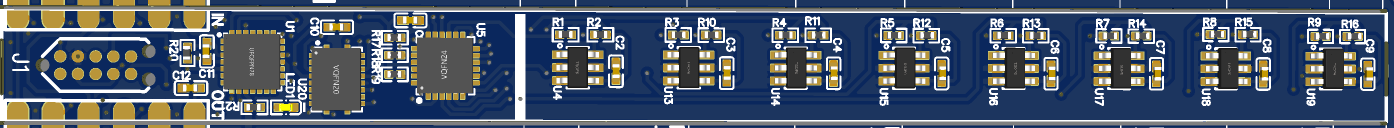
\includegraphics[width=8cm]{magcam_sensor_module.png}}
\caption{Sensor Slice with eight TLV493d sensors}
\label{magcam_sensor_module_fig}
\end{figure}

The sensor slice shown in Figure \ref{anpmagcam_sensor_module_fig_fig} consists of 8 TLV493d sensors spaced 8mm apart on an 8mm x 64mm PCB.
To build a larger sensor array, the golf finger pads of the board can be soldered to other similar boards in a daisy chain configuration.

The daisy chain design simplifies connectivity as multiple slices can be connected in a linear fashion, reducing complex wiring.
This approach simplifies expansion and troubleshooting, as new slices can be easily added or removed without disrupting the entire system.

In this way, an 8x8 sensor array can be built quickly, and the mechanical stability and alignment is ensured by the interconnection of the golf finger pads.

\subsection{Communication bus}

To ensure modularity and easy expandability of the sensor system, it is necessary to be able to integrate several sensor slices into the system.
On the electrical level, a CAN bus was implemented to connect the individual microprocessors to which up to 16 magnetic field sensors can be digitally connected to an overall system.

In addition to the bus system, a supply voltage and a separate synchronisation signal are necessary to enable automatic recognition of connected sensors. This is connected in a daisy chain between the slices.
This enables the microcontroller of a sensor slice to recognise whether it is integrated into a network and to register itself via the system bus.



\subsection{Powermanagement}

Each sensor slice also implements its own power management of the sensors, both at the hardware and software level, but this is optional.

Depending on the type of sensor used, the current flowing through the individual layers can influence its measurement result.
Therefore, the control logic and voltage converter components were placed separately from the sensors in the board layout.
In addition, individual sensors can be specifically supplied with voltage. This was implemented using a switchable power supply (PCF847). 
The software is later (when activated) able to activate only the sensor that is to be read out at the current time.
A disadvantage of this implementation, however, is that each sensor must be reconfigured after activating the power supply.
Depending on the selected sensor, this can take up to an additional 10ms per sensor measurement.




\subsection{Mechanical integration}

% 3d printed cases for magnet holders
%



%-----------------------------------------------------------------------------------------------------------------------------------------------
% Embedded System Software
\section{Embedded System Software}

\subsection{Automatic Sub-Sensor Detection}

Due to the modular hardware design, it is necessary for the software to be able to recognise the individual slices automatically.
without the user having to enter the number of connected slices in the software.

Due to the can-bus used, however, it is not possible to directly recognise the sequence of the modules and therefore the individual sensors cannot be directly addressed.
Through an additional auto-numbering sequence after the system start, all connected modules address themselves automatically.

\begin{figure}[htbp]
\centerline{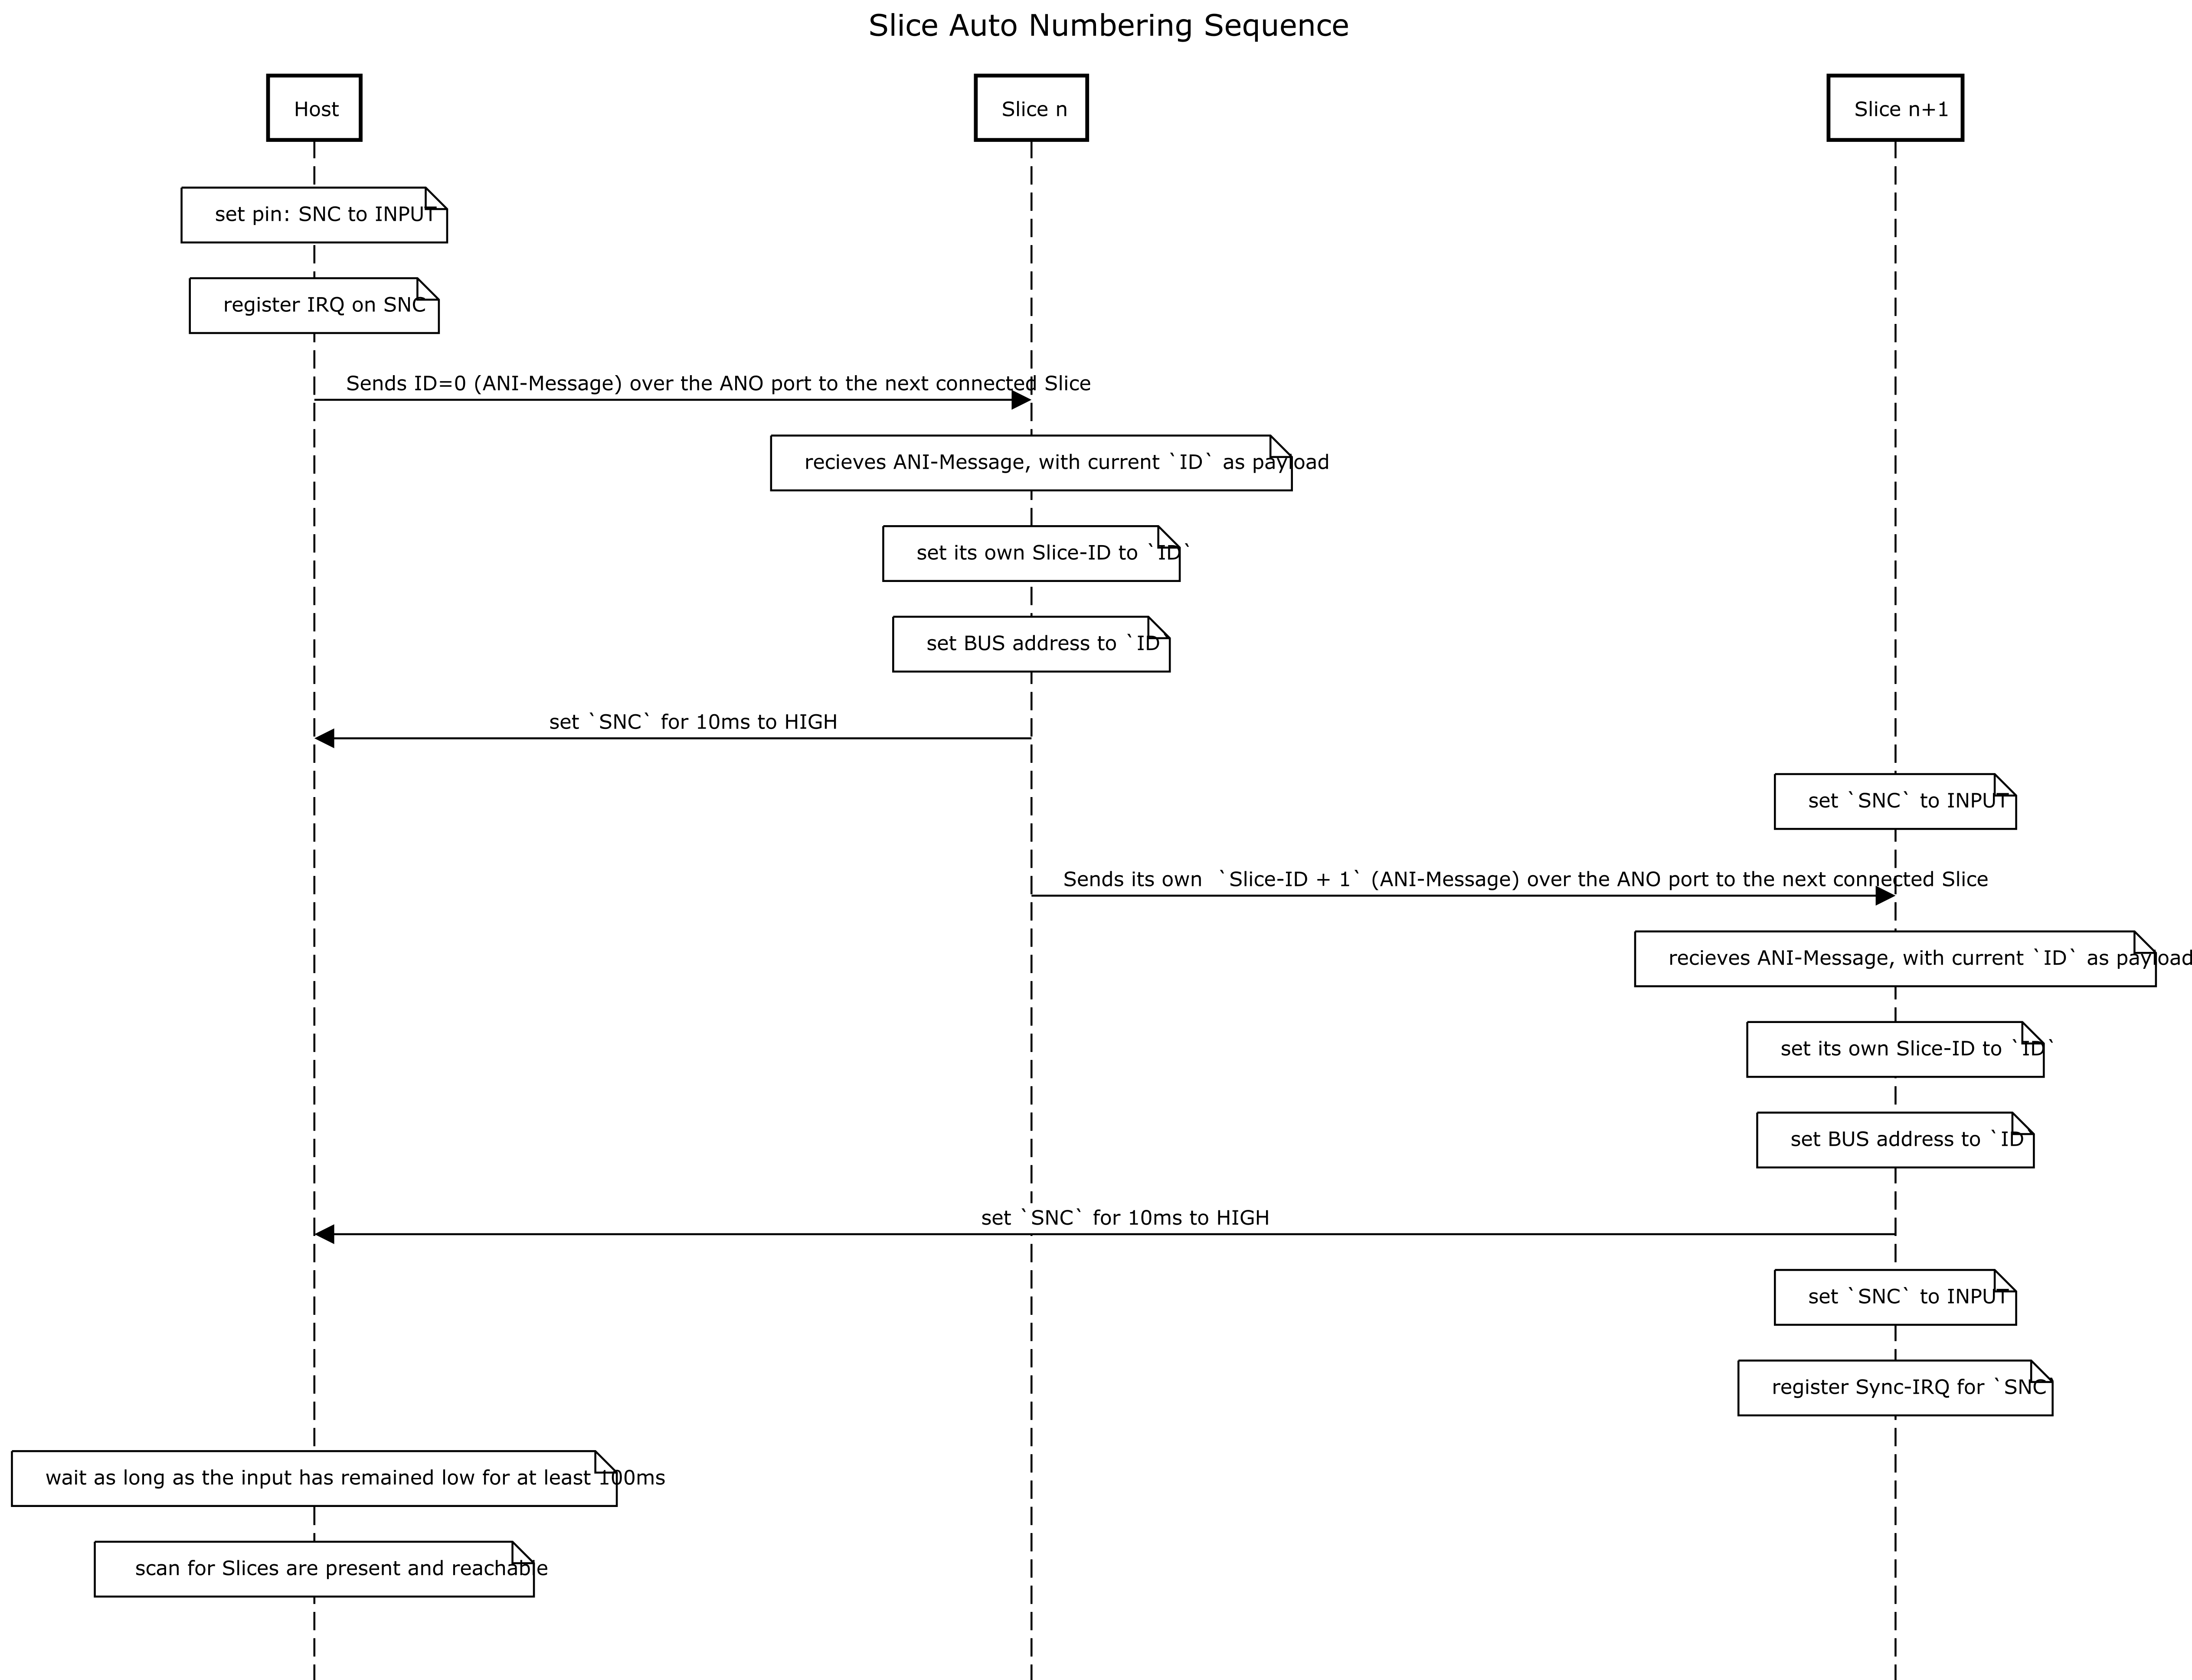
\includegraphics[width=8cm]{anp.png}}
\caption{Auto numbering protocol for multible connected slices}
\label{anp_fig}
\end{figure}

For this purpose, an additional clock line is used to carry out the protocol described (Figure \ref{anp_fig}). Later, this is used for synchronisation in order to have to use as few data lines as possible between the slices.
% each slice gets its own id and transmits +1 to the next

    


\subsection{Synchronisation}

In order to ensure synchronisation of all sensors in the array, in addition to the bus system used for data transmission, a clock line is shared between all sensors.
After performing the autonumbering procedure, the clock line, which was previously used as an autonumbering return channel, is reconfigured as a digital input.
This is done for all connected sensor modules except for the slices connected to the readout host system.
This module then specifies the read clock via this data line, which can be configured in the software.
All other sensors use this signal to trigger a readout interrupt.

This procedure also ensures that the rest of the system maintains a synchronised state even if sensor slices fail or are restarted.
Modules that fall into an out-of-sync status can thus be resynchronised directly after a synchronisation pulse.


%-----------------------------------------------------------------------------------------------------------------------------------------------
%Analysis Software Framework
\section{Analysis Software Framework}

The collection and subsequent processing of the data read from the sensor array is carried out on another computer system (host).
For this purpose, the Python framework is used, which was specially developed for the automated processing of magnetic field sensor data.
By adapting the sensor software on the basis of the documentation, a direct evaluation of the sensor is possible through the library.
Through the implemented auto-numbering routine and the feedback of this to the host software, each individual sensor is assigned to an individual measurement in the host software.


\subsection{Calibration strategy}


\subsection{Measurement Run}


\subsection{Data analysis pipeline}





cli einstellungen
+ ergebnis







%-----------------------------------------------------------------------------------------------------------------------------------------------
%Evaluation

\section{Evaluation}

\subsection{Comparison}
% mit mechanischen aufbau
% durch feste positionen nur zurückrechenbar

%-----------------------------------------------------------------------------------------------------------------------------------------------
%Conclusion

\section{Conclusion}


%-----------------------------------------------------------------------------------------------------------------------------------------------
\begingroup
\begin{thebibliography}{00}
%\setstretch{1.05}
\bibitem{modhhsf} Marcel Ochsendorf: Development of a hardware and software framework for the automated characterization of permanent magnets for low-field MRI systems. Available: \url{https://www.researchgate.net/publication/374388764_Development_of_a_permanent_magnet_characterization_framework_for_use_in_low-field_MRI_systems}, 17.11.2021.

\vskip 0.05in
\bibitem{MagneticReadoutProcessingLib} Marcel Ochsendorf: MagneticReadoutProcessing-Framework. \url{https://github.com/LFB-MRI/MagneticReadoutProcessing}, 17.11.2021


\end{thebibliography}
\endgroup

\end{document}


